\chapter{Systems Design for AI/ML at Scale}
\label{ch:systems-design-interviews}

\begin{quote}
\itshape
This chapter contains 40 systems design interview questions spanning AI infrastructure, ML platforms, and production AI systems. Each question includes a structured framework for approaching it, key design decisions, and the trade-offs interviewers expect you to discuss. Questions marked with $\star$ are particularly common.
\end{quote}

\vspace{0.5cm}


\section{How to Approach AI Systems Design Interviews}

AI systems design interviews differ from traditional systems design in three key ways:

\begin{enumerate}[leftmargin=*]
    \item \textbf{Probabilistic components}: You must design for non-deterministic behavior. A caching layer for LLM responses requires semantic similarity matching, not exact key lookup.
    \item \textbf{Cost as a first-class constraint}: LLM inference costs \$0.01--\$0.12 per request. At 10M requests/day, model selection and routing directly impact the P\&L.
    \item \textbf{Quality measurement}: You need an answer for ``How do you know the system is working?'' that goes beyond uptime and latency. Evaluation infrastructure is part of the system design.
\end{enumerate}

\subsection{The ACRES Framework}

For every systems design question, structure your answer using ACRES:

\begin{itemize}[leftmargin=*]
    \item \textbf{A}sk clarifying questions: Scope the problem. What scale? What latency requirements? What quality bar?
    \item \textbf{C}omponent design: Draw the high-level architecture. Identify the major components and their responsibilities.
    \item \textbf{R}easoning about trade-offs: For each major decision, discuss alternatives and justify your choice.
    \item \textbf{E}valuation strategy: How will you measure whether the system works? What metrics? What SLOs?
    \item \textbf{S}caling and failure modes: How does the system scale? What are the failure modes, and how do you handle them?
\end{itemize}


\section{RAG Systems}

\subsection{Q1: Design a Customer Support RAG System $\star$}

\textbf{Scenario}: Design a RAG-powered customer support system for a SaaS company with 50,000 help articles, 10,000 daily queries, and a requirement for 95\% answer accuracy.

\begin{figure}[H]
\centering
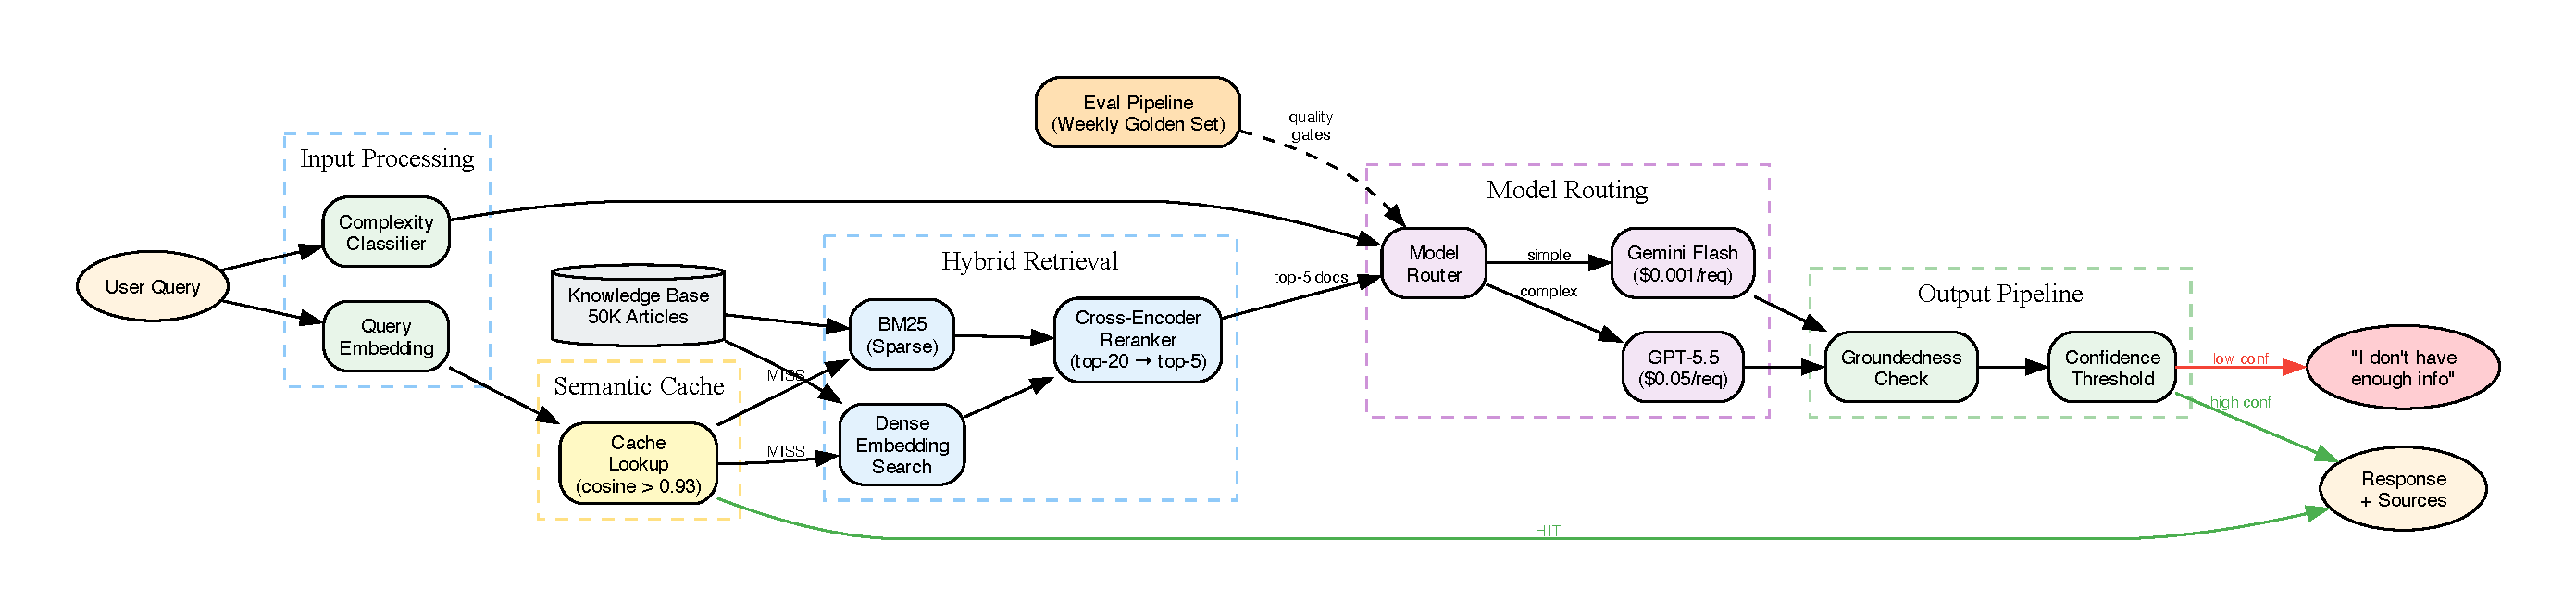
\includegraphics[width=\textwidth]{diagrams/ch17/rag-system.pdf}
\caption{Customer Support RAG architecture: semantic cache, hybrid retrieval, complexity-based model routing, and groundedness checking.}
\label{fig:rag-system}
\end{figure}

\textbf{Key design decisions}:
\begin{itemize}[leftmargin=*]
    \item \textbf{Chunking strategy}: Semantic chunking at section boundaries with metadata headers (product, version, category). Fixed-size chunks lose context at boundaries.
    \item \textbf{Retrieval}: Hybrid search (dense embeddings + sparse BM25). Dense catches semantic similarity; BM25 catches exact terminology. Reranker (cross-encoder) on top-20 candidates.
    \item \textbf{Model routing}: Simple queries (``how do I reset my password?'') to Gemini 3.5 Flash. Complex queries (multi-product, troubleshooting) to GPT-5.5. Route based on query complexity classifier.
    \item \textbf{Evaluation}: Groundedness metric (every claim must trace to a source document). Weekly golden dataset evaluation. A/B test query routing thresholds.
    \item \textbf{Failure mode}: Retrieval returns irrelevant documents $\to$ model hallucinates. Mitigation: confidence threshold on retrieval scores; below threshold, respond ``I don't have enough information to answer this.''
\end{itemize}

\textbf{Interviewer Follow-ups}:
\begin{itemize}[leftmargin=*]
    \item \textbf{Metrics \& SLOs}: Answer accuracy $\geq$ 95\% (weekly golden set), groundedness $\geq$ 98\%, p95 latency $<$ 3s, cache hit rate $>$ 25\%, retrieval relevance (MRR@5 $>$ 0.7).
    \item \textbf{Testing}: Golden dataset of 500 (question, expected\_answer, source\_document) triples. Automated nightly evals. Regression alerts when any category drops $>$2\%.
    \item \textbf{Traffic splitting}: Route 5\% of production traffic to a candidate model and compare quality scores. Promote via canary rollout.
    \item \textbf{Model routing logic}: Classifier trained on (query\_text, best\_model) pairs from offline evaluation. Retrain monthly as query distribution shifts.
    \item \textbf{Load balancing}: Requests distributed across retrieval replicas via round-robin. LLM calls use the model gateway with least-outstanding-requests routing.
\end{itemize}

\subsection{Q2: Multi-Tenant RAG Platform}

\textbf{Scenario}: Design a RAG platform that serves 500 enterprise customers, each with their own knowledge base (1K--100K documents). Customers must never see each other's data.

\textbf{Key design decisions}:
\begin{itemize}[leftmargin=*]
    \item \textbf{Tenant isolation}: Namespace-based isolation in the vector database (per-tenant collection/partition). Never mix embeddings across tenants in the same index.
    \item \textbf{Embedding model}: Shared embedding model across tenants (cost-efficient) vs. per-tenant fine-tuned embeddings (better quality for specialized domains).
    \item \textbf{Scale}: Most tenants are small. Use a tiered architecture: shared infrastructure for small tenants, dedicated resources for enterprise.
\end{itemize}

\subsection{Q3: Real-Time RAG with Streaming Data}

\textbf{Scenario}: Design a RAG system for a financial news service where the knowledge base updates continuously (new articles every few minutes) and queries must reflect the latest information.

\textbf{Key design decisions}:
\begin{itemize}[leftmargin=*]
    \item \textbf{Index freshness}: Streaming embedding pipeline---new documents are embedded and indexed within 2 minutes of publication
    \item \textbf{Temporal weighting}: Recent documents should be weighted higher in retrieval. Add a time-decay factor to similarity scores.
    \item \textbf{Cache invalidation}: Semantic cache must be invalidated when relevant documents are updated. Hash-based change detection per document.
\end{itemize}


\section{AI Application Architecture}

\subsection{Q4: Design a Model Gateway $\star$}

\textbf{Scenario}: Design a centralized API gateway that routes requests to multiple LLM providers (OpenAI, Anthropic, Google), handles failover, manages costs, and provides unified observability.

\begin{figure}[H]
\centering
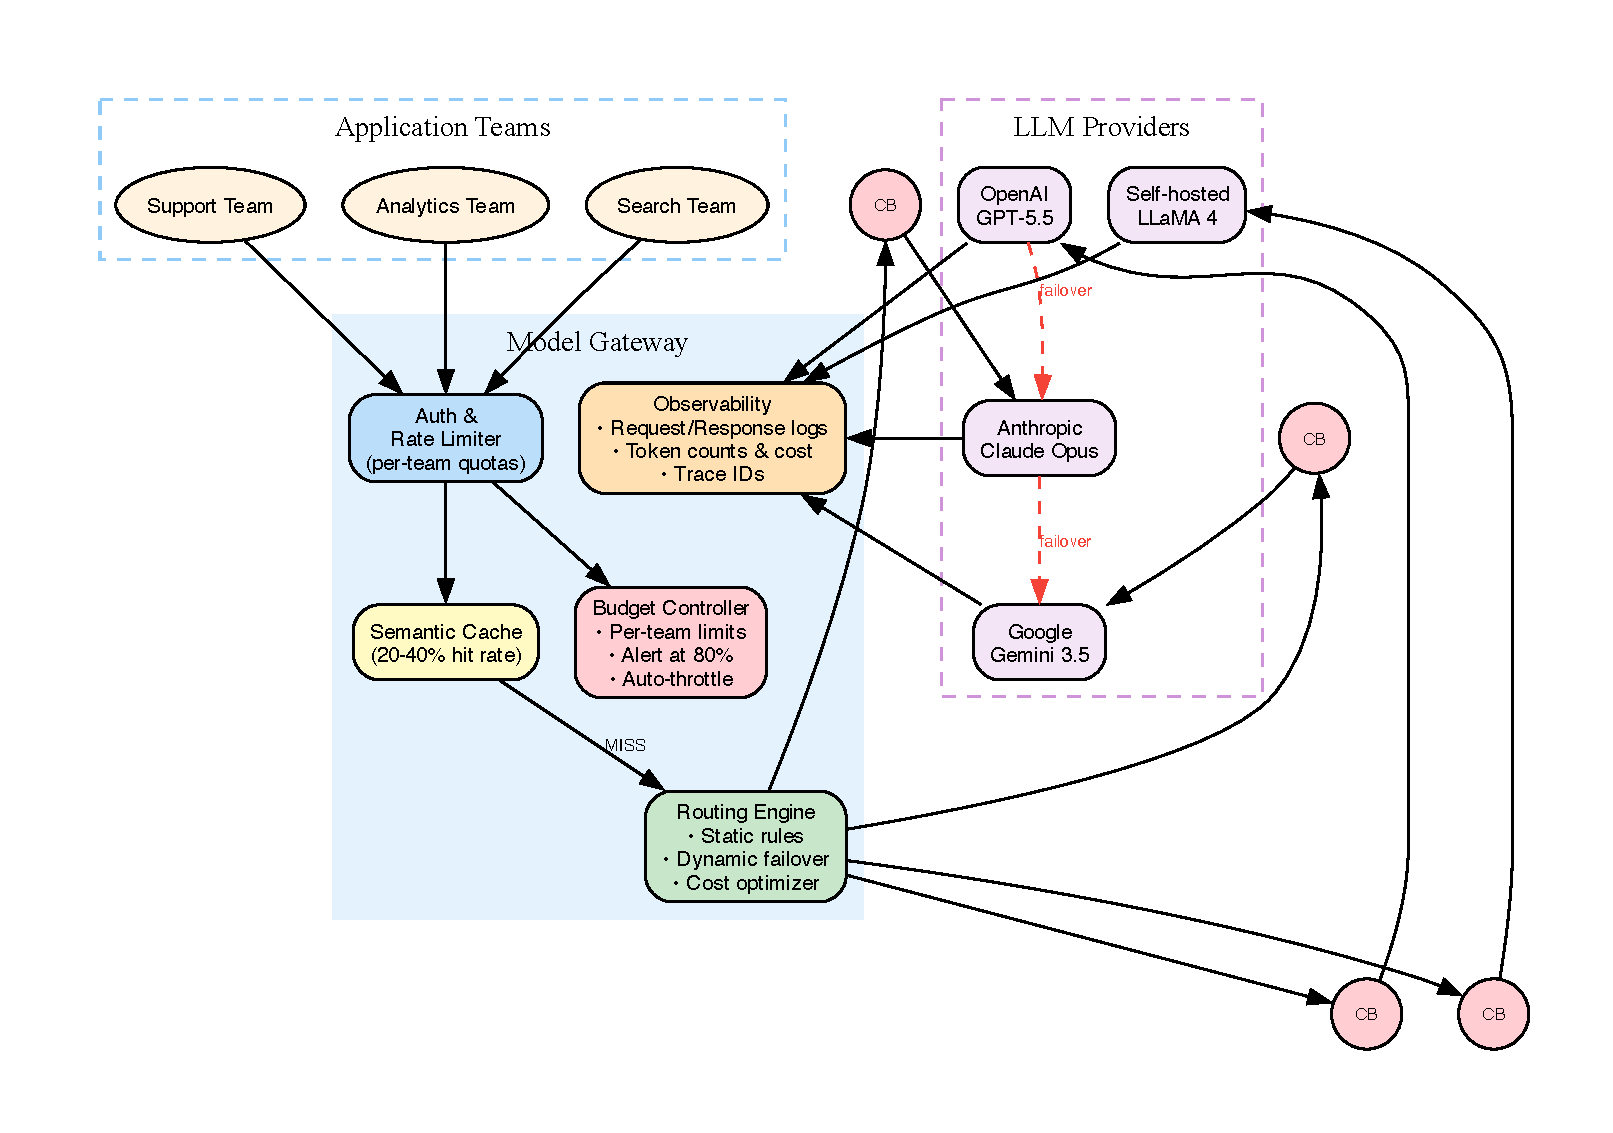
\includegraphics[width=0.9\textwidth]{diagrams/ch17/model-gateway.pdf}
\caption{Model Gateway: centralized routing with per-provider circuit breakers, semantic caching, budget control, and failover cascades.}
\label{fig:model-gateway}
\end{figure}

\textbf{Key design decisions}:
\begin{itemize}[leftmargin=*]
    \item \textbf{Routing strategy}: Static rules (feature X always uses provider Y) vs. dynamic routing (cost optimizer, quality optimizer, latency optimizer). In practice: static routing with dynamic failover.
    \item \textbf{Failover}: If provider A returns 5xx, automatically retry on provider B. Requires prompt portability across providers (not guaranteed---provider-specific prompt tuning).
    \item \textbf{Cost controls}: Per-team and per-feature token budgets. Real-time cost tracking. Alert and throttle when budgets are 80\% consumed.
    \item \textbf{Observability}: Log every request/response with model, latency, token count, cost, and a request ID that traces through the entire system.
    \item \textbf{Caching}: Semantic cache layer between the gateway and providers. Cache hit rate of 20--40\% on repetitive workloads reduces cost significantly.
\end{itemize}

\textbf{Interviewer Follow-ups}:
\begin{itemize}[leftmargin=*]
    \item \textbf{Metrics}: Per-provider latency (p50, p99), error rate, cost per request, cache hit rate, budget utilization per team, circuit breaker state transitions.
    \item \textbf{Testing}: Chaos engineering---inject failures into individual providers and verify failover works correctly. Load testing at 2$\times$ expected peak.
    \item \textbf{Traffic splitting}: A/B test new providers by routing 5\% of traffic and comparing quality. Consistent hashing on request ID ensures the same request always goes to the same variant.
    \item \textbf{Model migration}: When migrating from Provider A to Provider B, gradually shift traffic (5\% $\to$ 25\% $\to$ 50\% $\to$ 100\%) while monitoring quality and cost. Automated rollback if quality drops $>$2\%.
    \item \textbf{Load balancing}: Within a provider, use least-outstanding-requests routing. Across providers for the same tier, prefer the provider with the best current latency (adaptive routing).
\end{itemize}

\subsection{Q5: Design an LLM Evaluation Platform $\star$}

\textbf{Scenario}: Design an internal platform that allows teams to evaluate LLM outputs using golden datasets, rubric-based scoring, and A/B testing. Support 50 teams with different evaluation criteria.

\textbf{Key design decisions}:
\begin{itemize}[leftmargin=*]
    \item \textbf{Golden dataset management}: Versioned datasets in object storage. Schema: \code{(input, expected\_output, metadata, category)}. Teams own their datasets but share the infrastructure.
    \item \textbf{Evaluation pipeline}: Async job queue. Each evaluation run processes the full dataset, scores each case on the team's rubric, and produces a detailed report.
    \item \textbf{Judge management}: Centralized judge prompts per rubric dimension. Versioned alongside the evaluation datasets.
    \item \textbf{Comparison}: Side-by-side comparison of two model/prompt configurations on the same dataset. Statistical significance testing (Wilcoxon signed-rank).
\end{itemize}

\textbf{Interviewer Follow-ups}:
\begin{itemize}[leftmargin=*]
    \item \textbf{Metrics}: Evaluation throughput (cases/minute), judge consistency (inter-rater agreement when running the same case 3 times), time-to-report, per-team usage, cost per evaluation run.
    \item \textbf{Testing}: Validate judges: create cases with known-good and known-bad outputs. Assert the judge assigns high scores to good outputs and low scores to bad. Track judge drift over time.
    \item \textbf{Traffic splitting}: This \emph{is} the traffic splitting infrastructure. The eval platform gates model promotions: candidate model must beat baseline on all dimensions with $p < 0.05$ before promotion to production.
    \item \textbf{Model routing}: Route evaluation jobs to the appropriate compute tier---small golden datasets (100 cases) on shared compute, large regression suites (10K cases) on dedicated GPU instances.
    \item \textbf{Scale}: For 50 teams running daily evals, expect 50K+ LLM-as-Judge calls per day. Use batching, caching (same judge prompt + same output = deterministic score), and async processing to keep costs manageable.
\end{itemize}

\subsection{Q6: Design a Semantic Cache}

\textbf{Scenario}: Design a caching layer for LLM responses where cache hits are determined by semantic similarity rather than exact string match.

\textbf{Key design decisions}:
\begin{itemize}[leftmargin=*]
    \item \textbf{Similarity threshold}: At what cosine similarity do you consider two queries ``the same''? Too high (0.99) = low hit rate. Too low (0.85) = wrong answers served from cache. Typical: 0.92--0.95, tuned per use case.
    \item \textbf{Cache invalidation}: LRU + TTL. Cache entries expire after a configurable time. For knowledge-dependent queries, invalidate when the underlying knowledge base changes.
    \item \textbf{Embedding model}: Use a fast, small embedding model for cache lookup (not the production embedding model which may be larger and slower).
\end{itemize}


\section{AI Infrastructure}

\subsection{Q7: Design a Feature Store for ML $\star$}

\textbf{Scenario}: Design a feature store that serves both batch features (computed daily) and real-time features (computed on-demand) for a recommendation system processing 100K requests per second.

\textbf{Key design decisions}:
\begin{itemize}[leftmargin=*]
    \item \textbf{Dual storage}: Offline store (data warehouse, Parquet files) for batch features. Online store (Redis, DynamoDB) for real-time serving with p99 $<$ 10ms.
    \item \textbf{Feature computation}: Batch features via scheduled Spark/Flink jobs. Real-time features via stream processing (Kafka $\to$ Flink $\to$ Redis).
    \item \textbf{Point-in-time correctness}: Training must use features as they existed at prediction time (no future leakage). The feature store must support time-travel queries.
    \item \textbf{Feature registry}: Metadata catalog with feature definitions, owners, SLAs, and data lineage.
\end{itemize}

\subsection{Q8: Design a Model Serving Infrastructure}

\textbf{Scenario}: Design infrastructure to serve 20 different ML models with varying compute requirements (from small classifiers to 70B parameter LLMs) with a unified API.

\textbf{Key design decisions}:
\begin{itemize}[leftmargin=*]
    \item \textbf{Compute tiering}: Small models on CPU (cost-efficient). Medium models on single GPU. Large models on multi-GPU with tensor parallelism.
    \item \textbf{Batching}: Dynamic batching for GPU models---collect requests over a short window (10--50ms) and process as a batch for higher throughput.
    \item \textbf{Autoscaling}: Scale based on queue depth (pending requests) not CPU utilization. GPU models have a different scaling profile than CPU models.
    \item \textbf{Model versioning}: Blue-green deployment with traffic splitting. Every model has a version, and the routing layer controls which version serves traffic.
\end{itemize}

\subsection{Q9: Design a Training Pipeline for Continuous Fine-Tuning}

\textbf{Scenario}: Design a system that continuously fine-tunes a base model on new customer interaction data, evaluates the fine-tuned model, and promotes it to production if it meets quality gates.

\textbf{Key design decisions}:
\begin{itemize}[leftmargin=*]
    \item \textbf{Data pipeline}: Streaming new interactions into a data lake. Daily batch job curates training examples (quality filtering, deduplication, format conversion).
    \item \textbf{Training}: LoRA fine-tuning on curated data. Training triggered weekly or when $N$ new examples accumulate.
    \item \textbf{Evaluation}: Golden dataset evaluation with rubric scoring. Compare against current production model. Quality gate: new model must match or exceed baseline on every category.
    \item \textbf{Promotion}: Shadow deployment $\to$ canary rollout $\to$ full promotion. Automated rollback on quality regression.
\end{itemize}


\section{Agent Systems}

\subsection{Q10: Design a Code Review Agent $\star$}

\textbf{Scenario}: Design an AI agent that reviews pull requests for a large engineering organization ($\sim$500 engineers, $\sim$200 PRs per day). It should catch security issues, style violations, and suggest improvements.

\textbf{Key design decisions}:
\begin{itemize}[leftmargin=*]
    \item \textbf{Integration}: GitHub webhook triggers the agent on PR creation and update. Agent posts comments as a bot user.
    \item \textbf{Context}: The agent receives the diff, plus relevant files (imports, tests, related functions). Use codebase indexing to find relevant context automatically.
    \item \textbf{Multi-pass review}: Pass 1: Static analysis (linting, type checking). Pass 2: Security scan (SAST). Pass 3: LLM-based semantic review (architecture alignment, business logic correctness).
    \item \textbf{Feedback loop}: Track which agent comments are dismissed vs. addressed by developers. Use this signal to improve review quality over time.
    \item \textbf{Cost}: With 200 PRs/day averaging 300 lines each, estimate the token cost and model selection. Use a fast model for initial triage; escalate flagged issues to a frontier model.
\end{itemize}

\subsection{Q11: Design a Multi-Agent Research System}

\textbf{Scenario}: Design a system where multiple AI agents collaborate to research a topic: one agent searches the web, another reads and summarizes papers, a third synthesizes findings, and a coordinator manages the workflow.

\textbf{Key design decisions}:
\begin{itemize}[leftmargin=*]
    \item \textbf{Coordination}: Hierarchical---a coordinator agent decomposes the research question, assigns subtasks, collects results, and synthesizes.
    \item \textbf{Communication}: Structured messages between agents (task description, constraints, output format). Use the A2A protocol.
    \item \textbf{Termination}: The coordinator decides when enough evidence has been gathered. Budget limits prevent unbounded research.
    \item \textbf{Quality}: A critic agent reviews the synthesis for factual accuracy, unsupported claims, and logical coherence.
\end{itemize}


\section{Data Systems for AI}

\subsection{Q12: Design an Embedding Pipeline at Scale $\star$}

\textbf{Scenario}: You need to embed 50 million documents (averaging 2,000 tokens each) and keep the index updated as documents are added, modified, and deleted.

\textbf{Key design decisions}:
\begin{itemize}[leftmargin=*]
    \item \textbf{Batch processing}: Initial embedding via distributed GPU workers (Spark/Ray). Estimate: 50M docs × 2K tokens × embedding cost. Optimize with batching.
    \item \textbf{Incremental updates}: Content-hash-based change detection. Only re-embed documents whose content hash has changed. This reduces daily update cost by 80--90\%.
    \item \textbf{Chunking}: Chunk before embedding. Each document produces 2--10 chunks. Total index size: 100M--500M vectors.
    \item \textbf{Vector database selection}: At 100M+ vectors, purpose-built databases (Qdrant, Pinecone, Weaviate) outperform pgvector significantly. Consider sharding strategy.
\end{itemize}

\subsection{Q13: Design a Data Labeling Platform}

\textbf{Scenario}: Design a platform for labeling training data for an NLP model. Support 100 annotators, quality control (inter-annotator agreement), and active learning (prioritize labeling the most informative examples).

\textbf{Key design decisions}:
\begin{itemize}[leftmargin=*]
    \item \textbf{Quality control}: Assign each example to 2--3 annotators. Compute inter-annotator agreement (Cohen's kappa). Flag disagreements for expert review.
    \item \textbf{Active learning}: Use model uncertainty to prioritize which examples to label next. Label the examples the model is most uncertain about---this maximizes information gain per label.
    \item \textbf{Annotation interface}: Task-specific UI (text classification, NER, sequence labeling). Keyboard shortcuts for speed.
\end{itemize}


\section{Production AI Systems}

\subsection{Q14: Design a Content Moderation System $\star$}

\textbf{Scenario}: Design a system that moderates user-generated content on a social platform (10M posts per day) for hate speech, misinformation, and policy violations.

\textbf{Key design decisions}:
\begin{itemize}[leftmargin=*]
    \item \textbf{Tiered approach}: Tier 1: Fast classifier (fine-tuned BERT, $<$10ms) screens all content. Tier 2: LLM review for flagged content (explanation + category). Tier 3: Human review for edge cases and appeals.
    \item \textbf{Latency}: Tier 1 must be real-time ($<$50ms) so content is moderated before it's visible. Tier 2 can be async (minutes).
    \item \textbf{Feedback loop}: Human decisions from Tier 3 become training data for Tier 1 classifier, continuously improving automated moderation.
\end{itemize}

\subsection{Q15: Design a Recommendation System with LLM Explanations}

\textbf{Scenario}: Design a product recommendation system that provides natural language explanations for each recommendation (``We recommend this because...'').

\textbf{Key design decisions}:
\begin{itemize}[leftmargin=*]
    \item \textbf{Decoupled architecture}: The recommendation engine (collaborative filtering / embeddings) runs independently from the explanation generator (LLM). Don't use the LLM for ranking---it's too slow and expensive.
    \item \textbf{Explanation generation}: Feed the LLM the user's profile, the recommended item's features, and the recommendation reason (from the ML model). Generate a personalized explanation.
    \item \textbf{Caching}: Explanation templates for common recommendation reasons. LLM-generated explanations cached by (user segment, item category, recommendation reason).
\end{itemize}


\section{Reliability and Observability}

\subsection{Q16: Design an AI Incident Response System}

\textbf{Scenario}: Design a system that detects AI quality regressions in production, diagnoses the root cause, and triggers appropriate response actions.

\textbf{Key design decisions}:
\begin{itemize}[leftmargin=*]
    \item \textbf{Detection}: Statistical process control on rubric scores. CUSUM (cumulative sum) charts for detecting gradual drift. Z-score alerts for sudden drops.
    \item \textbf{Diagnosis}: Automated root cause analysis: Was there a recent deployment? Model version change? RAG index update? Input distribution shift?
    \item \textbf{Response}: Automated: rollback to last known good configuration. Manual: page on-call engineer with diagnosis context.
\end{itemize}

\subsection{Q17: Design an LLM Cost Optimization System}

\textbf{Scenario}: Your company spends \$500K/month on LLM API calls across 50 teams. Design a system that reduces costs by 40\% without degrading quality.

\textbf{Key design decisions}:
\begin{itemize}[leftmargin=*]
    \item \textbf{Model routing}: Classify query complexity and route simple queries to cheap models (Gemini 3.5 Flash: \$0.001/request) instead of expensive models (GPT-5.5: \$0.05/request)
    \item \textbf{Semantic caching}: 25--35\% hit rate on repetitive workloads eliminates those API calls entirely
    \item \textbf{Prompt optimization}: Audit prompts for unnecessary verbosity. Shorter system prompts = fewer input tokens
    \item \textbf{Batch processing}: Move non-real-time workloads to batch API (50\% discount from most providers)
    \item \textbf{Self-hosting}: For high-volume, stable workloads, self-host an open-source model. Break-even analysis: volume threshold where self-hosting is cheaper than API.
\end{itemize}


\section{Questions 18--40: Brief Prompts}

The following questions are presented as brief prompts to practice structuring your approach using the ACRES framework.

\begin{enumerate}[leftmargin=*]
    \item[Q18.] Design a plagiarism detection system using embeddings for a university with 100K student submissions per semester
    \item[Q19.] Design a multilingual chatbot that serves users in 20 languages with a single underlying model
    \item[Q20.] Design a real-time fraud detection system that uses both ML classifiers and LLM reasoning for complex cases
    \item[Q21.] Design a document summarization pipeline that processes 1M legal documents into structured summaries
    \item[Q22.] Design a search system that combines keyword search, semantic search, and LLM-powered query understanding
    \item[Q23.] Design a CI/CD pipeline for ML models with automated testing, evaluation, and promotion
    \item[Q24.] Design an A/B testing framework for LLM-powered features with statistical significance testing
    \item[Q25.] Design a data pipeline that processes and deduplicates a 100TB web crawl for LLM pre-training
    \item[Q26.] Design a model registry that tracks model lineage, hyperparameters, and evaluation results
    \item[Q27.] Design a privacy-preserving inference system that processes sensitive medical data without exposing it to a third-party LLM provider
    \item[Q28.] Design a knowledge graph construction pipeline that extracts entities and relationships from unstructured text at scale
    \item[Q29.] Design a speech-to-text transcription pipeline that handles 10K concurrent audio streams
    \item[Q30.] Design a prompt management system that supports versioning, A/B testing, and rollback across 100 features
    \item[Q31.] Design a multi-modal AI system that answers questions about product images (``What material is this made of?'')
    \item[Q32.] Design an autonomous coding agent that can implement features from Jira tickets end-to-end
    \item[Q33.] Design a personalized email generation system for a marketing platform with 10M users
    \item[Q34.] Design a log analysis system that uses LLMs to identify root causes from production logs
    \item[Q35.] Design a competitive intelligence system that monitors competitor websites, news, and social media
    \item[Q36.] Design an LLM-powered data validation pipeline that checks incoming data against business rules expressed in natural language
    \item[Q37.] Design a federated learning system for training a model across 1,000 hospital sites without sharing patient data
    \item[Q38.] Design a real-time translation system for a video conferencing platform with 100 concurrent sessions
    \item[Q39.] Design an AI-powered code migration tool that converts a legacy Java codebase to modern Python
    \item[Q40.] Design an end-to-end observability platform for AI/ML systems that correlates model quality metrics with infrastructure metrics
\end{enumerate}


\section{Hard System Design: GPU \& Inference Infrastructure}
\label{sec:hard-gpu}

These questions are common at Google DeepMind, Meta FAIR, and any company building or operating large-scale inference infrastructure. They require back-of-envelope calculations and deep understanding of GPU constraints.

\subsection{Q41: Design a High-Throughput LLM Inference Service $\star$}

\textbf{Scenario (Google DeepMind/Meta)}: Design a serving system for a 70B parameter LLM that handles 100K requests per second with p99 latency under 2 seconds. The model must be served on a fleet of 8$\times$H100 GPU nodes.

\begin{figure}[H]
\centering
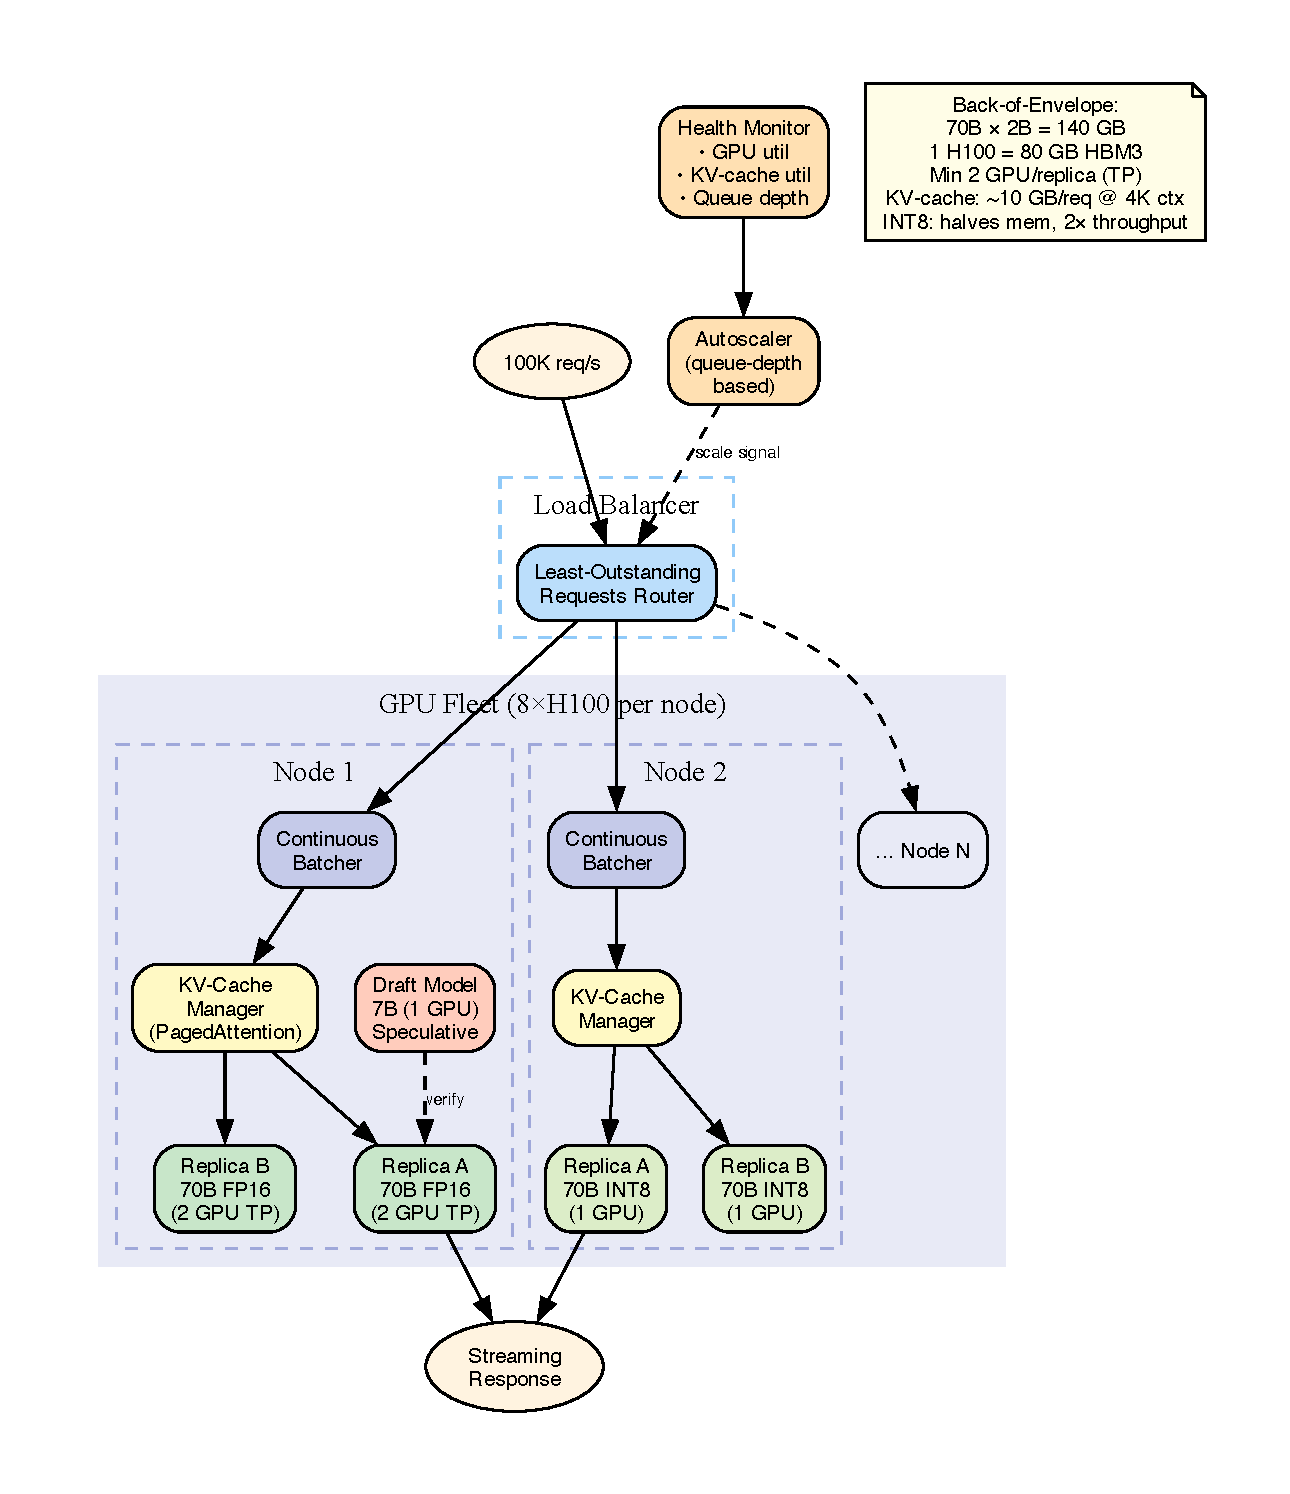
\includegraphics[width=\textwidth]{diagrams/ch17/llm-inference.pdf}
\caption{High-throughput LLM inference: continuous batching, PagedAttention KV-cache, speculative decoding, and queue-depth autoscaling.}
\label{fig:llm-inference}
\end{figure}

\textbf{Back-of-envelope}: 70B params $\times$ 2 bytes (FP16) = 140 GB model weights. One H100 has 80 GB HBM3. Minimum 2 GPUs per replica with tensor parallelism. With 8 GPUs per node, run 4 replicas per node (or 2 replicas with pipeline parallelism for better latency).

\textbf{Key design decisions}:
\begin{itemize}[leftmargin=*]
    \item \textbf{KV-cache management}: The KV cache for a 70B model at 4K context length is $\sim$10 GB per request. With concurrent requests, KV-cache memory is the binding constraint, not compute. Use PagedAttention (vLLM) to avoid fragmentation.
    \item \textbf{Batching strategy}: Continuous batching---don't wait for all requests in a batch to finish before accepting new ones. As each request completes (EOS token), its slot is immediately available for a new request.
    \item \textbf{Quantization trade-off}: INT8 quantization halves memory, doubles throughput, but costs 1--3\% quality. Run the evaluation suite on quantized model; if quality meets threshold, deploy quantized.
    \item \textbf{Speculative decoding}: Use a small draft model (7B) to predict 3--5 tokens, then verify with the 70B model. Acceptance rate $\sim$70--80\%, giving $\sim$2$\times$ throughput for free.
    \item \textbf{Load balancing}: Least-outstanding-requests routing, not round-robin. GPU inference workloads have variable latency per request (depends on output length).
\end{itemize}

\textbf{Failure modes}: GPU OOM from KV-cache exhaustion $\to$ reject new requests when KV-cache utilization $>$ 90\%. GPU failure $\to$ health check and automatic node replacement. Straggler nodes $\to$ request replication to fastest-available node.

\textbf{Interviewer Follow-ups}:
\begin{itemize}[leftmargin=*]
    \item \textbf{Metrics \& SLOs}: Requests/second, p50/p99 latency, GPU utilization, KV-cache utilization, batch fill rate, tokens/second throughput, time-to-first-token (TTFT).
    \item \textbf{Testing}: Load testing with realistic prompt length distribution (not uniform). Soak testing for 24+ hours to detect memory leaks. Chaos testing: kill a GPU mid-inference and verify graceful recovery.
    \item \textbf{Traffic splitting}: Run quantized and full-precision models side-by-side. Route 10\% of traffic to quantized, compare quality using LLM-as-Judge. If quality is within 1\%, migrate to quantized (2$\times$ throughput).
    \item \textbf{Scaling}: Autoscale on queue depth, not GPU utilization (GPU util is a trailing indicator). Target: queue depth $<$ 10 requests per replica. Pre-warm new nodes with model weights before routing traffic.
\end{itemize}

\subsection{Q42: Design a Distributed Training Platform $\star$}

\textbf{Scenario (Google DeepMind/Meta FAIR)}: Design a platform that trains 100B+ parameter models across 1,024 GPUs. It must support: data parallelism, tensor parallelism, pipeline parallelism, checkpointing (every 30 min), and automatic recovery from node failures.

\textbf{Key design decisions}:
\begin{itemize}[leftmargin=*]
    \item \textbf{Parallelism strategy}: 3D parallelism. Data parallelism across nodes (8-way), tensor parallelism within nodes (8 GPUs), pipeline parallelism across node groups (16 stages). Total: $8 \times 8 \times 16 = 1024$ GPUs.
    \item \textbf{Communication}: All-reduce for gradient synchronization (NCCL). Overlap communication with computation---while layer $N+1$ is computing, layer $N$'s gradients are being all-reduced.
    \item \textbf{Checkpointing}: Async checkpointing to distributed storage. Only rank 0 per data-parallel group writes weights. Use ZeRO-style sharding to reduce checkpoint size.
    \item \textbf{Fault tolerance}: The ``straggler problem''---if one GPU is 10\% slower, all 1,024 GPUs wait. Detection: per-step timing alerts. Mitigation: hot spare nodes, automatic worker replacement, elastic training.
    \item \textbf{Job scheduling}: Priority queue with preemption. Long training jobs ($\sim$weeks) need fair-share scheduling. Support spot/preemptible instances for cost reduction.
\end{itemize}

\textbf{Interviewer Follow-ups}:
\begin{itemize}[leftmargin=*]
    \item \textbf{Metrics \& SLOs}: Training throughput (samples/second), GPU utilization ($>$85\% target), checkpoint success rate, mean time to recovery (MTTR) after node failure, communication overhead (\% of step time in all-reduce).
    \item \textbf{Testing}: Test fault tolerance: kill a random node mid-training, verify auto-recovery from last checkpoint within 5 minutes. Test scaling: add 128 GPUs to a running job and verify throughput scales linearly.
    \item \textbf{Cost optimization}: Use spot instances for data-parallel workers (replaceable). Use on-demand for pipeline-parallel stages (failure is more disruptive). Estimated savings: 60--70\% with spot.
    \item \textbf{Debugging}: The ``loss spike'' problem---how do you debug a loss spike at step 50,000? Log gradient norms per layer, learning rate schedule, data batch composition. Enable deterministic replay: given a checkpoint and data ordering, reproduce the exact training state.
    \item \textbf{Load balancing}: Within a training job, all GPUs must be identically loaded. A slow GPU (thermal throttling, memory error) slows the entire job. Continuous health monitoring with automatic replacement.
\end{itemize}

\subsection{Q43: Design a Multi-Region Inference Deployment}

\textbf{Scenario}: Design a global LLM inference service deployed across 5 regions (US-East, US-West, EU, Asia, South America) with data residency requirements: EU user data must not leave EU, all other regions can share.

\textbf{Key design decisions}:
\begin{itemize}[leftmargin=*]
    \item \textbf{Routing}: GeoDNS for region selection + application-level routing for data residency enforcement. EU requests always routed to EU cluster.
    \item \textbf{Model synchronization}: Same model version across all regions. Coordinated deployment: update one region at a time (canary), verify quality gates, then proceed.
    \item \textbf{Cache strategy}: Per-region semantic caches (no cross-region cache sharing to preserve data residency). Prompt templates can be shared globally.
    \item \textbf{Failover}: If EU capacity is exhausted, queue requests (don't route to US). For non-EU regions, overflow to nearest available region.
\end{itemize}


\section{Hard System Design: Safety-Critical AI Systems}
\label{sec:hard-safety}

These questions are common at Anthropic, OpenAI, and any company building consumer-facing AI. They test your ability to design systems where safety is not an afterthought but a first-class architectural concern.

\subsection{Q44: Design an AI Safety Guardrails Pipeline $\star$}

\textbf{Scenario (Anthropic)}: Design the input/output safety pipeline for a consumer-facing AI assistant. It must: filter harmful inputs, detect prompt injection, classify output safety, handle adversarial users, and comply with regional content regulations (EU, US, China).

\begin{figure}[H]
\centering
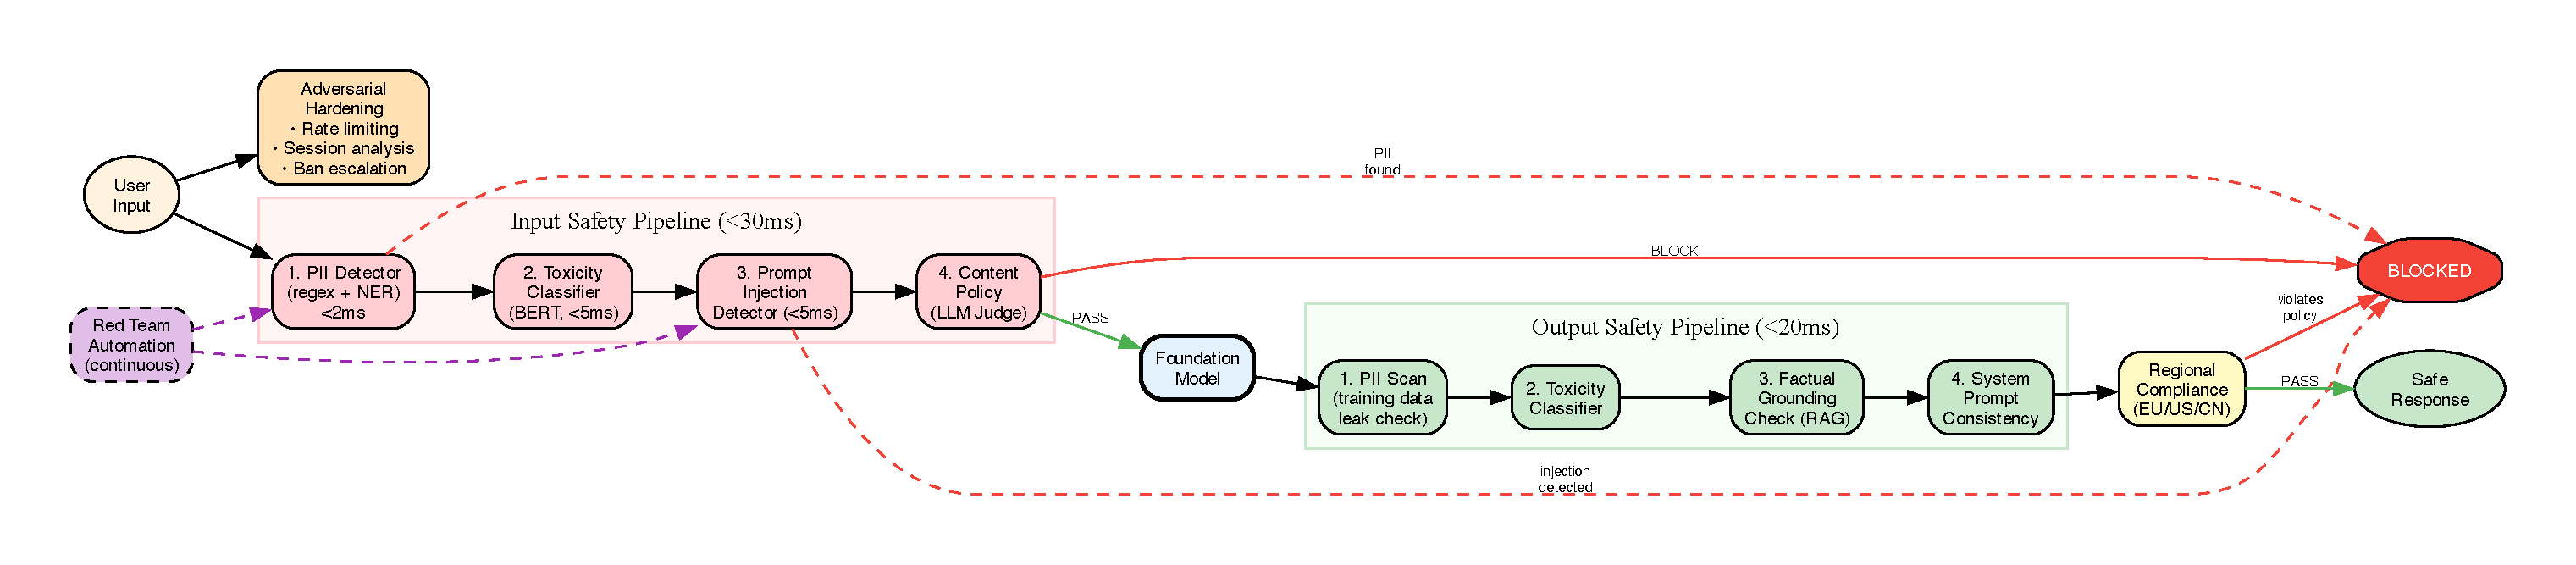
\includegraphics[width=\textwidth]{diagrams/ch17/safety-pipeline.pdf}
\caption{AI Safety Guardrails: cascaded input/output classifiers with regional compliance, adversarial hardening, and automated red-team testing.}
\label{fig:safety-pipeline}
\end{figure}

\textbf{Key design decisions}:
\begin{itemize}[leftmargin=*]
    \item \textbf{Input pipeline}: Classifier cascade: (1) PII detector (regex + NER model), (2) toxicity classifier (fine-tuned BERT, $<$5ms), (3) prompt injection detector (fine-tuned classifier on known attack patterns), (4) content policy classifier (LLM-as-Judge for edge cases). Each stage can block or flag.
    \item \textbf{Output pipeline}: (1) PII scan of output (prevent model from leaking training data), (2) toxicity classifier, (3) factual grounding check (for RAG), (4) output consistency check (does the output contradict the system prompt's constraints?).
    \item \textbf{Regional compliance}: Policy configuration per region. A response that's acceptable in US may be required to include disclaimers in EU or be blocked entirely in other jurisdictions.
    \item \textbf{Adversarial hardening}: Rate limiting per user, session-level behavior analysis (detect users who are systematically probing for jailbreaks), and automatic ban escalation.
    \item \textbf{Cost}: The full safety pipeline adds 15--30ms latency and 5--10\% cost overhead. This is non-negotiable for consumer AI.
\end{itemize}

\textbf{Interviewer Follow-ups}:
\begin{itemize}[leftmargin=*]
    \item \textbf{Metrics}: False positive rate (legitimate queries blocked) $<$ 0.01\%, false negative rate (harmful content passed) $<$ 0.1\%, safety pipeline latency (p99 $<$ 30ms), block rate by category, jailbreak attempt rate.
    \item \textbf{Testing}: Red-team evaluation suite of 1,000+ adversarial prompts across 20 attack categories. Automated nightly runs. Track attack success rate as a north-star metric (target: $<$ 0.01\%).
    \item \textbf{Traffic splitting}: When updating safety classifiers, run old and new classifiers in parallel on 100\% of traffic. Alert on disagreements. Promote new classifier only when disagreement rate is $<$ 0.1\% and all disagreements are manual-reviewed.
    \item \textbf{Model routing}: Safety-critical applications (healthcare, finance) use the strictest safety pipeline. Internal tools may use a lighter pipeline for lower latency.
    \item \textbf{Load balancing}: Safety classifiers are lightweight (BERT-sized). Deploy on CPU with horizontal scaling. Autoscale based on request rate, not latency.
\end{itemize}

\subsection{Q45: Design an AI Alignment Evaluation System}

\textbf{Scenario (Anthropic/OpenAI)}: Design a system that continuously evaluates whether a deployed AI model is behaving within its alignment specifications. Detect: hallucination, refusal regression, boundary violations, and emergent harmful behaviors.

\textbf{Key design decisions}:
\begin{itemize}[leftmargin=*]
    \item \textbf{Red-team automation}: Continuously generate adversarial prompts using a separate LLM (the ``attacker model''). Test the production model against these prompts and flag any responses that violate safety specifications.
    \item \textbf{Refusal calibration}: Track the refusal rate over time. A sudden drop in refusals on harmful topics indicates a potential alignment regression. A sudden increase in refusals on benign topics indicates over-restriction.
    \item \textbf{Behavioral drift}: Embed model responses weekly and compute distributional shift (KL divergence) against a baseline. Large distributional shifts trigger a manual review.
    \item \textbf{Escalation}: Automated alerts for clear violations; human review queue for ambiguous cases; executive escalation for systematic alignment failures.
\end{itemize}

\subsection{Q46: Design a Regulated Healthcare AI System}

\textbf{Scenario}: Design an AI system that assists doctors by summarizing patient records and suggesting possible diagnoses. The system must comply with HIPAA, maintain an audit trail, and never provide a definitive diagnosis (only suggestions with confidence levels).

\textbf{Key design decisions}:
\begin{itemize}[leftmargin=*]
    \item \textbf{Data handling}: PHI (Protected Health Information) never leaves the hospital's VPC. Self-hosted model (LLaMA 4 or similar) on-premises. No API calls to external LLM providers.
    \item \textbf{Audit trail}: Every model interaction is logged immutably: input (patient ID anonymized for logs), output, model version, timestamp, and the clinician who requested it.
    \item \textbf{Output constraints}: The system always generates confidence levels (``high confidence'', ``consider'', ``unlikely''). It explicitly states that it is not providing a diagnosis and that clinical judgment is required.
    \item \textbf{Evaluation}: Clinical accuracy validated against a panel of physicians using a gold-standard case set. FDA regulatory pathway (if applicable) requires pre-market clinical validation.
\end{itemize}


\section{Hard System Design: Financial \& Payment AI}
\label{sec:hard-financial}

These questions are common at Stripe, Square, and financial services companies. They test your ability to combine ML with strict correctness, regulatory, and latency requirements.

\subsection{Q47: Design an AI-Powered Fraud Detection Pipeline $\star$}

\textbf{Scenario (Stripe)}: Design a real-time fraud detection system that processes 50,000 payment transactions per second. It must: make a decision within 100ms, maintain a false positive rate below 0.1\%, adapt to new fraud patterns within hours, and provide explainable decisions for regulatory compliance.

\textbf{Key design decisions}:
\begin{itemize}[leftmargin=*]
    \item \textbf{Multi-stage architecture}: Stage 1: Rules engine ($<$1ms, catches known patterns). Stage 2: Real-time ML model (gradient-boosted trees, $<$10ms). Stage 3: LLM reasoning for ambiguous cases ($<$2s, async---hold the payment briefly if needed).
    \item \textbf{Feature engineering}: Real-time features (velocity, device fingerprint, IP geolocation) computed via stream processing. Historical features (user spending patterns, merchant reputation) from the feature store.
    \item \textbf{Model retraining}: Online learning with concept drift detection. When fraud patterns shift (detected via performance monitoring), trigger retraining on recent labeled data within hours.
    \item \textbf{Explainability}: SHAP values for the ML model. LLM generates natural language explanation of the decision for compliance reports (``This transaction was flagged because the velocity exceeded 3$\sigma$ from the user's 90-day average and originated from a new country'').
    \item \textbf{Feedback loop}: Chargebacks (confirmed fraud) and customer disputes (false positives) are labeled training data. Time lag: chargebacks arrive 30--90 days after the transaction.
\end{itemize}

\textbf{Interviewer Follow-ups}:
\begin{itemize}[leftmargin=*]
    \item \textbf{Metrics \& SLOs}: Fraud detection rate $>$ 99.5\%, false positive rate $<$ 0.1\%, decision latency $<$ 100ms (p99), model staleness $<$ 4 hours (time since last retraining).
    \item \textbf{Testing}: Shadow mode for new models---run alongside production without acting on decisions. Compare predictions. A/B test with held-out traffic (1\% of transactions use the candidate model). Measure precision/recall at the production threshold.
    \item \textbf{Traffic splitting}: Route 1\% of transactions to the candidate model. Both models make decisions, but only the production model's decision is acted upon. Compare FPR/FNR offline.
    \item \textbf{Load balancing}: Stage 1 (rules) and Stage 2 (ML) must be on the hot path ($<$100ms total). Deploy in every region. Stage 3 (LLM) is async---use a distributed task queue.
    \item \textbf{Model routing}: Route obvious fraud (high-confidence ML) directly to block. Route borderline cases to LLM reasoning for nuanced analysis. Route clear non-fraud directly to allow.
\end{itemize}

\subsection{Q48: Design an AI Transaction Categorization System}

\textbf{Scenario (Stripe/Plaid)}: Design a system that automatically categorizes bank transactions (``AMZN MARKETPLACE 123'' $\to$ ``Shopping / Online Retail'') for 500M transactions per day across 10,000 merchants.

\textbf{Key design decisions}:
\begin{itemize}[leftmargin=*]
    \item \textbf{Hybrid approach}: Rule-based matching for known merchant names ($\sim$70\% of transactions). ML classifier for the long tail ($\sim$25\%). LLM for truly ambiguous cases ($\sim$5\%).
    \item \textbf{Merchant resolution}: Merchant description strings are noisy (``SQ *JOE'S COFFEE'', ``PAYPAL *JOESCOFFEESHOP''). Fuzzy matching + learned merchant embeddings to resolve variations of the same merchant.
    \item \textbf{Cost optimization}: At 500M transactions/day, even \$0.001 per LLM call = \$500K/day. Use the LLM only for the 5\% that rules and ML can't handle. Cache LLM categorizations by normalized merchant description.
\end{itemize}


\section{Hard System Design: Developer Tools AI}
\label{sec:hard-devtools}

These questions are common at GitHub, GitLab, JetBrains, and any company building AI-powered developer tools.

\subsection{Q49: Design GitHub Copilot $\star$}

\textbf{Scenario (GitHub)}: Design an AI code completion system integrated into IDEs. It must: provide inline completions with $<$200ms latency, support 50+ programming languages, handle multi-file context, respect .gitignore and private repository boundaries, and improve over time from user acceptance/rejection signals.

\textbf{Key design decisions}:
\begin{itemize}[leftmargin=*]
    \item \textbf{Context construction}: The hardest problem. Current file + imports + recently edited files + project structure. Context budget: 8K--16K tokens. Use a retrieval step to find the most relevant code snippets from the repository.
    \item \textbf{Model architecture}: Fast, small model for single-line completions (speculative generation). Larger model for multi-line/function completions. Client-side model for latency-critical completions in the future.
    \item \textbf{Latency budget}: $<$200ms end-to-end. Network: $\sim$50ms. Model inference: $\sim$100ms. Context construction: $\sim$50ms. This means aggressive caching of model state (KV-cache per session) and precomputed context.
    \item \textbf{Feedback loop}: Track acceptance rate per language, per project type, per completion length. Use accepted completions as positive training signal and rejections as negative signal. But beware: users reject completions for many reasons (distraction, already knew the answer), so rejection is a weak negative signal.
    \item \textbf{Privacy}: Repository code sent to the inference server must be handled with the same security as the repository itself. Enterprise customers require: data residency, no training on their code, audit logs.
\end{itemize}

\textbf{Interviewer Follow-ups}:
\begin{itemize}[leftmargin=*]
    \item \textbf{Metrics}: Completion acceptance rate (CAR), completions per session, latency (p50 $<$ 100ms, p99 $<$ 200ms), user retention, daily active completions, cost per completion.
    \item \textbf{Testing}: Offline evaluation on a held-out corpus: does the model predict the next line correctly? Metric: exact-match rate, BLEU-4 on multi-line completions. Online A/B test: measure acceptance rate between model versions.
    \item \textbf{Traffic splitting}: New model deployed to 5\% of users (not requests---user-level assignment for consistent experience). Monitor acceptance rate and session length. Promote at 10\% $\to$ 50\% $\to$ 100\% over 2 weeks.
    \item \textbf{Real-time model selection}: Shorter completions (1 line) use a fast, small model. Multi-line completions use a larger model. If the user is typing fast (likely not looking at completions), suppress suggestions entirely to save cost.
    \item \textbf{Load balancing}: Sticky sessions per user for KV-cache reuse. New users assigned to the server with the lowest load. Preemptive context computation: start building context when the user opens a file, before they start typing.
\end{itemize}

\subsection{Q50: Design an Agentic Coding System}

\textbf{Scenario}: Design a system where an AI agent receives a feature request (from a Jira ticket or natural language description) and autonomously: analyzes the codebase, creates a plan, implements the code changes across multiple files, writes tests, runs them, and submits a pull request.

\textbf{Key design decisions}:
\begin{itemize}[leftmargin=*]
    \item \textbf{Codebase understanding}: Index the repository: code embeddings for semantic search, AST parsing for structural navigation, dependency graph for impact analysis.
    \item \textbf{Planning}: The agent generates a multi-step plan before writing code. The plan is reviewed (by a human or a critic agent) before execution begins.
    \item \textbf{Execution loop}: For each step: generate code $\to$ run linter $\to$ run tests $\to$ if failure, analyze error and retry (max 3 times) $\to$ proceed to next step.
    \item \textbf{Safety}: The agent operates in a sandboxed environment (container). No network access, no access to secrets, no access to production databases. All file modifications are staged in a branch.
    \item \textbf{Quality gate}: Before submitting the PR: all tests pass, code coverage doesn't decrease, no new linting errors, a critic agent reviews the changes for architectural alignment.
\end{itemize}

\textbf{Interviewer Follow-ups}:
\begin{itemize}[leftmargin=*]
    \item \textbf{Metrics}: PR merge rate (what \% of agent-generated PRs are merged without modification?), time to first review, lines changed per task, test pass rate on first attempt, retry rate per step, cost per PR.
    \item \textbf{Testing}: Run the agent on a curated set of 100 historical tickets (where the actual PR is known). Compare the agent's changes against the human's changes. Measure: functional equivalence, code quality (linting, complexity), and test coverage.
    \item \textbf{Traffic splitting}: Start with ``suggestion mode'' (agent generates PR but doesn't auto-merge). Graduate to ``draft PR mode'' (auto-creates draft, human reviews). Finally, ``auto-merge for trivial changes'' (typos, dependency bumps).
    \item \textbf{Model routing}: Simple tasks (rename variable, update constant) use a fast, cheap model. Complex tasks (new feature, refactor) use a frontier model with longer context. The task classifier runs before the agent starts.
    \item \textbf{Safety}: The sandbox must prevent: arbitrary code execution, network access, credential theft. Use gVisor or Firecracker for OS-level isolation. All generated code goes through the same security review pipeline as human code.
\end{itemize}


\section{Hard System Design: Knowledge \& Enterprise AI}
\label{sec:hard-enterprise}

These questions are common at LinkedIn, Salesforce, and enterprise SaaS companies building AI features at scale.

\subsection{Q51: Design LinkedIn's AI-Powered Job Matching $\star$}

\textbf{Scenario (LinkedIn)}: Design a system that matches job seekers with relevant job postings. It processes: 200M user profiles, 20M active job postings, and must serve 50K match requests per second with personalized rankings.

\textbf{Key design decisions}:
\begin{itemize}[leftmargin=*]
    \item \textbf{Two-stage retrieval}: Stage 1: Candidate generation via embedding similarity (user profile embedding vs. job embedding). Return top 1,000 candidates in $<$10ms using ANN index. Stage 2: Reranking with a cross-encoder model that considers fine-grained features (skills match, experience level, location, salary range).
    \item \textbf{Embedding model}: Train on implicit signals (applications, saves, views) and explicit signals (rejections, ``not interested''). Update embeddings daily.
    \item \textbf{Cold start}: New users with sparse profiles: use content-based features (resume text, skills listed). New job postings: use job description embedding + employer reputation.
    \item \textbf{Fairness}: The ranking must not discriminate on protected attributes. Audit for demographic parity and equality of opportunity across gender, age, and race. Debias embeddings if needed.
\end{itemize}

\textbf{Interviewer Follow-ups}:
\begin{itemize}[leftmargin=*]
    \item \textbf{Metrics}: Application rate (did the user apply?), interview conversion rate, time-to-fill (for job posters), result diversity score, fairness audit pass rate.
    \item \textbf{Testing}: Offline recall@100 on historical application data. Online A/B test: does the new ranking model increase application rate? Fairness audit: ensure no statistically significant difference in recommendation quality across demographic groups.
    \item \textbf{Traffic splitting}: User-level A/B assignment (not request-level). 10\% of users see candidate ranking for 2 weeks. Measure application rate and user satisfaction survey scores.
    \item \textbf{Model routing}: Premium users get the full cross-encoder reranking (expensive). Free-tier users get embedding-only matching (cheaper, slightly lower quality).
    \item \textbf{Load balancing}: Embedding index sharded by geography. US users query US shards (lower latency, more relevant results). Cross-shard queries for remote-job seekers.
\end{itemize}

\subsection{Q52: Design an Enterprise Knowledge Management System}

\textbf{Scenario}: Design an AI system that indexes an enterprise's entire knowledge base (Confluence, Slack, Google Drive, email---500M documents across 10K employees) and answers questions using RAG. Data access must respect document-level permissions.

\textbf{Key design decisions}:
\begin{itemize}[leftmargin=*]
    \item \textbf{Permission-aware retrieval}: The biggest challenge. When User A queries the system, retrieval must filter to only documents User A has access to. Options: (a) pre-filter in the vector DB query (metadata filter), (b) post-filter retrieved results against the permission system, (c) per-user indexes (doesn't scale).
    \item \textbf{Multi-source ingestion}: Each data source has different APIs, auth mechanisms, and update patterns. Build source-specific connectors with incremental sync (process only new/modified documents since last sync).
    \item \textbf{Staleness}: Enterprise documents change frequently. The system must detect stale information and prioritize recent versions. Show confidence indicators and source dates to users.
    \item \textbf{Data sensitivity}: Some documents are confidential. The LLM response must not leak confidential information to unauthorized users, even indirectly (e.g., ``I can't share that document, but the answer to your question is...'' still leaks information).
\end{itemize}

\subsection{Q53: Design an AI-Powered Data Analytics Copilot}

\textbf{Scenario}: Design a system where business analysts can ask questions in natural language (``What were our top-performing products in Q3 by region?'') and get SQL queries, visualizations, and narrative insights generated automatically.

\textbf{Key design decisions}:
\begin{itemize}[leftmargin=*]
    \item \textbf{Schema understanding}: The LLM needs to understand the database schema (tables, columns, relationships, business terminology). Provide a schema description document in the system prompt, enriched with column-level descriptions and example values.
    \item \textbf{SQL generation}: Use the Validator-Corrector Proxy pattern---generate SQL, validate syntax, execute in a read-only sandbox, check for reasonable result sizes, and present to the user. If the query fails, feed the error back to the LLM for correction.
    \item \textbf{Safety}: Read-only database access. Query timeout (30s). Result size limits (10K rows max). No access to PII columns without explicit authorization.
    \item \textbf{Evaluation}: Maintain a golden dataset of (question, expected SQL, expected answer) triples. Evaluate SQL correctness (same results as expected SQL, not necessarily same syntax) and answer quality.
\end{itemize}


\section{Hard System Design: Frontier Challenges}
\label{sec:hard-frontier}

These questions represent the cutting edge of AI systems engineering---the problems that top labs are actively working on. They are intentionally under-specified; strong candidates drive the scoping.

\subsection{Q54: Design a Self-Improving AI System $\star$}

\textbf{Scenario}: Design a system where an AI model continuously improves itself using feedback from production interactions. Users rate responses, and the system uses this feedback to fine-tune the model, evaluate the fine-tuned version, and deploy it---all automatically.

\textbf{Critical trade-offs}:
\begin{itemize}[leftmargin=*]
    \item \textbf{Data quality}: User ratings are noisy (users rate based on expectation, not quality). Filter: require minimum rating volume per category, discard outliers, weight ratings by user reliability score.
    \item \textbf{Catastrophic forgetting}: Fine-tuning on recent data may degrade performance on older tasks. Mitigation: always include a representative sample of the original training data in each fine-tuning batch.
    \item \textbf{Safety drift}: As the model self-improves, it may optimize for user satisfaction at the expense of safety (users might rate harmful but entertaining responses highly). Automated safety evaluation must gate every deployment.
    \item \textbf{Feedback delay}: The time between deployment and receiving enough feedback to fine-tune is days to weeks. The system must be patient and avoid overfitting to small sample sizes.
\end{itemize}

\subsection{Q55: Design a Real-Time Voice AI Agent}

\textbf{Scenario}: Design an AI agent that conducts real-time voice conversations (phone calls). End-to-end latency from user speech to AI speech must be $<$500ms. The agent must handle: interruptions, hold/transfer, multi-turn context, and emotional tone detection.

\textbf{Key design decisions}:
\begin{itemize}[leftmargin=*]
    \item \textbf{Pipeline}: Speech-to-Text ($\sim$100ms) $\to$ LLM reasoning ($\sim$200ms) $\to$ Text-to-Speech ($\sim$100ms) = 400ms total. Each component must be streaming to overlap processing.
    \item \textbf{Interruption handling}: If the user starts speaking while the AI is speaking, immediately stop TTS output, flush the STT buffer, and process the interruption.
    \item \textbf{Turn-taking}: Detect end-of-turn via silence detection (300ms pause) + prosodic cues (falling intonation). Avoid responding too early (cutting off the user) or too late (awkward silence).
    \item \textbf{Emotional intelligence}: Tone classifier on the STT output to detect frustration, confusion, or urgency. Adjust the agent's response style (more empathetic for frustrated users, more concise for urgent requests).
\end{itemize}

\subsection{Q56: Design a Multi-Modal Search Engine}

\textbf{Scenario}: Design a search engine that accepts queries in any modality (text, image, voice, video clip) and returns results from a multi-modal corpus (documents, images, videos, audio). Cross-modal search must work: a text query should find relevant images, and an image query should find relevant text documents.

\textbf{Key design decisions}:
\begin{itemize}[leftmargin=*]
    \item \textbf{Unified embedding space}: Use a multi-modal embedding model (CLIP-like) that maps all modalities into a shared vector space. Text, images, and video frames are all represented as vectors in the same space.
    \item \textbf{Query processing}: Text queries embedded directly. Image queries: embed the image + optionally generate a text description (captioning) and embed that too (multi-vector query). Voice queries: STT first, then text embedding.
    \item \textbf{Index design}: Single ANN index for all modalities (since they share the same embedding space). Metadata filters for modality-specific search (``only show me videos'').
    \item \textbf{Reranking}: Cross-modal reranker that considers modality-specific relevance signals. An image result for a text query needs visual relevance; a text result for an image query needs descriptive precision.
\end{itemize}

\subsection{Q57: Design a Model Marketplace}

\textbf{Scenario}: Design a platform where model creators can publish, version, and monetize their fine-tuned models, and consumers can discover, evaluate, and deploy them via API. Think ``npm for AI models.''

\textbf{Key design decisions}:
\begin{itemize}[leftmargin=*]
    \item \textbf{Model registry}: Version control for model weights, training configs, evaluation results, and license information.
    \item \textbf{Evaluation}: Standardized benchmarks that all models are evaluated on. Consumer-defined evaluation on custom datasets before purchase.
    \item \textbf{Serving}: The platform handles inference infrastructure. Consumers get an API endpoint; they don't manage GPUs. The platform handles scaling, failover, and cost optimization.
    \item \textbf{Monetization}: Pay-per-token pricing set by model creators. Revenue split between platform and creator. Usage analytics for creators.
    \item \textbf{Security}: Model weights are never downloadable (for proprietary models). Inference runs on the platform's infrastructure. Prevent model extraction attacks (limit query volume, add watermarking to outputs).
\end{itemize}

\subsection{Q58: Design a Continent-Scale Data Deduplication Pipeline}

\textbf{Scenario (Meta/Google)}: You are preparing training data for the next pre-training run. You have 200TB of web crawl data and need to: (a) deduplicate at the document level (exact and near-duplicate), (b) deduplicate at the paragraph level (copied passages), (c) filter low-quality content, and (d) do this within a 72-hour processing window.

\textbf{Key design decisions}:
\begin{itemize}[leftmargin=*]
    \item \textbf{Exact dedup}: Hash each document (SHA-256). Group by hash. Trivially parallelizable. Remove exact duplicates: typically eliminates 20--30\% of the corpus.
    \item \textbf{Near-duplicate}: MinHash + LSH (Locality-Sensitive Hashing). Compute MinHash signatures (128 hashes per document), band into 20 bands of 6--7 hashes each. Documents in the same band with high Jaccard similarity ($>$0.8) are near-duplicates. Eliminates another 10--15\%.
    \item \textbf{Paragraph-level}: n-gram suffix array approach. Build a suffix array on 13-grams. Passages that share $>$200 consecutive tokens with other documents are flagged.
    \item \textbf{Quality filtering}: Perplexity-based filtering (use a small LM to score each document; very high perplexity = garbage text). Heuristic filters: document length, character-to-word ratio, presence of boilerplate markers.
    \item \textbf{Compute}: 200TB at 72 hours = 2.7 TB/hour. Distribute across 500--1000 worker nodes. The bottleneck is the LSH step (requires cross-document comparison).
\end{itemize}

\subsection{Q59: Design a Prompt Injection Defense System $\star$}

\textbf{Scenario (Anthropic/OpenAI)}: Design a system-wide defense against prompt injection for a platform where third-party applications use your LLM via API. Attacks come from: (a) direct user input, (b) documents retrieved by RAG, (c) tool outputs (web pages, API responses), and (d) multi-turn conversation manipulation.

\textbf{Key design decisions}:
\begin{itemize}[leftmargin=*]
    \item \textbf{Input classification}: Fine-tuned classifier on known injection patterns. Updated weekly with new attack vectors. False positive rate must be $<$0.01\% (legitimate queries must not be blocked).
    \item \textbf{Instruction hierarchy}: The model must be trained (via RLHF/DPO) to prioritize system prompt instructions over user instructions over tool-output instructions. This is an alignment problem, not just a filtering problem.
    \item \textbf{Canary tokens}: Embed invisible canary strings in the system prompt. If the model outputs the canary string, it indicates the system prompt has been extracted. Alert and block the user.
    \item \textbf{Tool output sandboxing}: Tool outputs (web pages, API responses) are treated as untrusted. Wrap them in explicit delimiters and instruct the model to treat them as data, not as instructions.
    \item \textbf{Red team automation}: Continuously generate novel injection attacks and test the defense system. Track the attack success rate over time as the defense metric.
\end{itemize}

\textbf{Interviewer Follow-ups}:
\begin{itemize}[leftmargin=*]
    \item \textbf{Metrics}: Injection detection rate $>$ 99.9\%, false positive rate $<$ 0.01\%, canary extraction rate (target: 0), time to detect new attack vectors $<$ 24 hours.
    \item \textbf{Testing}: Automated red-team pipeline: generate 1,000 novel injection attempts weekly using an attacker LLM. Measure bypass rate. Manual red-team exercises quarterly.
    \item \textbf{Traffic splitting}: When updating the injection classifier, run old and new in parallel. Only block with the old classifier; log disagreements from the new classifier for offline review.
    \item \textbf{Load balancing}: Injection classifiers are fast ($<$5ms). Co-locate with the API gateway to avoid additional network hops.
\end{itemize}

\subsection{Q60: Design a Foundation Model Training Data Curation Pipeline $\star$}

\textbf{Scenario (Google DeepMind/Meta/Anthropic)}: Design the end-to-end pipeline that curates training data for a new foundation model. The pipeline must: source data from 50+ domains, ensure legal compliance (copyright, PII), balance domain representation, apply quality filters, and produce tokenized training sequences ready for the training infrastructure.

\textbf{Key design decisions}:
\begin{itemize}[leftmargin=*]
    \item \textbf{Data sourcing}: Web crawl (CommonCrawl), curated datasets (Wikipedia, books, academic papers), code repositories (GitHub), and proprietary data (licensed content). Each source has different licensing, quality, and domain characteristics.
    \item \textbf{Legal compliance}: PII detection and redaction (regex + NER model). Copyright filtering: remove content matching known copyrighted works (using near-duplicate detection against a reference corpus). Opt-out compliance: respect robots.txt and data removal requests.
    \item \textbf{Domain balancing}: The final training mix is a critical hyperparameter. Typical: 50\% web, 15\% code, 15\% books/papers, 10\% curated knowledge, 10\% conversation/instruction data. Over-representation of web data leads to ``internet-brained'' models; under-representation leads to poor generality.
    \item \textbf{Quality pipeline}: Language detection $\to$ content classification $\to$ perplexity filtering $\to$ toxicity filtering $\to$ deduplication (exact + near) $\to$ domain classification $\to$ sampling.
    \item \textbf{Tokenization and packing}: Tokenize with the chosen tokenizer (BPE). Pack documents into training sequences of \code{max\_seq\_len} tokens with document boundary tokens. Random shuffling across domains within each training batch.
    \item \textbf{Versioning and reproducibility}: The entire pipeline must be reproducible. Every filter, threshold, and sampling decision must be versioned. The training data mix is an artifact that is tracked alongside the model weights.
\end{itemize}

\textbf{Interviewer Follow-ups}:
\begin{itemize}[leftmargin=*]
    \item \textbf{Metrics}: Corpus size after each filter stage, deduplication ratio, PII detection recall ($>$99\%), domain distribution match vs. target mix, processing throughput (TB/hour).
    \item \textbf{Testing}: Unit tests for each filter (known PII strings, known copyrighted passages). Integration test: run the full pipeline on a 1 GB sample and verify output characteristics (domain distribution, avg. document length, PII absence).
    \item \textbf{Traffic splitting}: For the training pipeline, this translates to data mix ablations---train small models on different domain mixes and compare benchmark performance to find the optimal mix.
    \item \textbf{Load balancing}: Distribute processing across worker nodes by data source. The web crawl (largest source) gets the most workers. Use consistent hashing by document URL for reproducible deduplication.
\end{itemize}

